\section{Statistical Identities and Scope}\label{app:proofs}
\subsection{Normal envelope and continuous Gaussian comparison}
Here is a proof of Proposition~\ref{prop:normal}. Write $q(t)=z\sqrt{1+t^2}$ and
$F(t)=\Phi(q(t)-t)+\Phi(q(t)+t)-1$. For $t>0$, set
$c=q'(t)=zt/\sqrt{1+t^2}$. Direct differentiation gives
\[
F'(t)=\phi(q-t)\{(c-1)+(c+1)e^{-2qt}\}.
\]
For $c\ge1$ this is nonnegative. For $0<c<1$, nonnegativity is equivalent to
\[
\operatorname{arctanh}(c)\ge qt=\frac{c}{1-c^2/z^2}.
\]
The absolutely convergent power series have coefficients $1/(2j+1)$ and
$z^{-2j}$, respectively. Since $z^2\ge3$ and $3^j\ge2j+1$ for all
integers $j\ge0$, the inequality holds termwise. Thus $F$ is nondecreasing
and $F(t)\ge F(0)=2\Phi(z)-1$. Symmetry handles negative mean; zero variance
follows directly. This is a sufficient range of $z$, not a claim that
$\sqrt3$ is the sharp boundary.

For $G=\A\A^*$, $a=\A\ell$, $L=\norm\ell^2$, and fixed positive covariance
$\Sigma$, completing a quadratic yields
\begin{align}
v(w)&=w^\top\Sigma w+\tau^2\norm{\ell-\A^*w}^2,\\
w_*&=(G+\Sigma/\tau^2)^{-1}a,\\
v(w_*)&=\tau^2(L-a^\top w_*).
\end{align}
These are the joint Gaussian conditional mean weights and variance for an
isonormal prior. With $\Sigma=I$, $\tau=B$, and fixed weights, the worst
absolute class bias is $b=B\norm{\ell-\A^*w}$. The proposition implies
$z\sqrt{v(w)}$ covers every allowed fixed density at level $1-\alpha$ for
$z=z_{1-\alpha/2}\ge\sqrt3$. The statement even holds for nonoptimal fixed
$w$ if the variance expression on the first line is used. That expression
must not be relabeled the exact posterior variance at an unfinished solve.
The implication does not require drawing a density from the Gaussian prior.
Conversely, posterior calibration averaged over a prior and fixed-density
uniform calibration are different statements in general. The matched result
here prevents claiming that their distinction alone favors our audit.

An isonormal process $W(f)$ has covariance $E[W(f)W(g)]=\ip f g$ for
$f,g\in H$. Joint Gaussian laws of $W(\ell)$ and finitely many observation
functionals exist. Identity covariance on infinite-dimensional $H$ has
infinite trace, so there is no associated finite-energy random element of
$H$ with that covariance. This is a generalized-process comparison, not a
claim that all prior draws belong to the bounded density class.

\subsection{Optimization, duality, and numerical error}
The sum-width problem has dual
\begin{equation}
\min_w z\norm w+B\norm{\ell-\A^*w}
=\max_{\norm v\le B,\,\norm{\A v}\le z}\ip\ell v.
\end{equation}
Express the residual norm as the support function of the radius-$B$ ball.
Minimizing $z\norm w-w^\top\A v$ gives zero when $\norm{\A v}\le z$
and minus infinity otherwise. The continuous norm objective and finite
observation space satisfy the usual convex duality qualification. A simple
feasible certificate is $v=th$ with $h=\ell-\A^*w$ and
$t=\min(B/\norm h,z/\norm{\A h})$, interpreting a zero denominator as
no constraint. It gives lower bound $t(L-w^\top a)$. We report the gap for
this sum objective; selecting a folded-normal width afterwards does not
make that width globally optimal.

For $H_\tau=G+\Sigma/\tau^2$ and residual $r=H_\tau w-a$, completing the
same quadratic gives
\begin{equation}\label{eq:solvegap}
v(w)-v(w_*)=\tau^2r^\top H_\tau^{-1}r.
\end{equation}
If $FF^\top\preceq G$ is a truncated pivoted-Cholesky approximation and
$\Sigma\succeq I$, put $P=FF^\top+I/\tau^2$. Then
$P\preceq H_\tau$ and the right-hand side is at most
$\tau^2r^\top P^{-1}r$. Adding a residual diagonal to this preconditioner
need not preserve this ordering. If an approximate Gram action has residual
error at most $e$, then
\[
\sqrt{r^\top P^{-1}r}\le
\sqrt{r_Q^\top P^{-1}r_Q}+\tau e.
\]
We use this as a numerical optimization diagnostic, with the analytic
integration remainder below. Roundoff and transform approximation are not
validated enclosures, and a small variance gap alone does not bound mean
error for every possible observed image vector.

\section{Continuous Fourier Computation}\label{app:continuous}
\subsection{Adjoint and target integrals}
Integrating the two conjugate expansions of a real Fourier field yields
Equation~\eqref{eq:sincgram}. For a unit-mass Gaussian component of center
$\mu$ and standard deviation $\sigma_\ell$, its one-dimensional transform
truncated to the unit interval is
\begin{align}
&e^{-2\pi i k\mu-2\pi^2\sigma_\ell^2k^2}\nonumber\\
&\quad\times[\Phi((1/2-\mu)/\sigma_\ell+2\pi i\sigma_\ell k)\nonumber\\
&\hspace{45pt}-\Phi((-1/2-\mu)/\sigma_\ell+2\pi i\sigma_\ell k)].
\end{align}
Products over coordinates and linear combinations over target components
give $\A\ell$. Gaussian-product integrals give $\norm\ell^2$. The sign
of the transform follows the convention in the main text. Independent
tensor quadrature and a conic formulation using the joint Hilbert Gram of
$[\ell,\A_1^*,\ldots,\A_m^*]$ check these expressions and the optimizer.

For $r$ Gauss--Legendre nodes on a unit interval, let
\[
C_r=\frac{(r!)^4}{(2r+1)((2r)!)^3},\quad
E_r=\sum_{a=1}^3 C_r(4\pi M_a)^{2r},\quad
M_a=\max_j|k_{ja}|.
\]
The classical derivative remainder \citep{dlmfquadrature} gives, for the
positive tensor weights $\omega_t$,
\begin{equation}
\left|\norm{f_w}^2-\sum_t\omega_t f_w(x_t)^2\right|
\le E_r\left(\sum_j|c_j|\right)^2.
\end{equation}
Indeed, the exponential expansion of $f_w^2$ has coordinate frequencies at
most $2M_a$ and coefficient absolute sum at most $(\sum_j|c_j|)^2$.
Apply the one-dimensional remainder in each coordinate and telescope the
three integration/quadrature operators; their positive weights sum to one.
Likewise,
\begin{equation}
\norm{(G-G_Q)w}\le\sqrt2 E_r\norm{C/\sigma}_2\sum_j|c_j|.
\end{equation}
We add the scalar error to the squared residual and the vector error to the
dual feasibility denominator. This preserves a continuous primal/dual
bracket in real arithmetic. At radius five, order 40 gives a kernel
remainder no larger than $3.21\times10^{-23}$ before coefficient scaling.
Two type-3 transforms apply $G_Q$. Requested FINUFFT tolerance $10^{-12}$ is
checked against independent sinc Grams; it is not a rigorous floating-point
bound. Cached plans change setup overhead, not the mathematical operator.

\subsection{Constant-cell generators and spectral Gaussian pilots}
An orthonormal constant-cell coefficient has density value $d^{3/2}$ on a
cell of volume $d^{-3}$. Its transform includes the exact cell sinc product
$\prod_a\operatorname{sinc}(k_a/d)$ and the half-cell phase relative to a
centered FFT grid. Target coefficients use Gaussian CDF differences. Thus
a piecewise constant simulation density is projected as a continuous
function, not as point samples. Generator grids of 64 and pilot grids of
24 have the same continuous norm convention; unit-normalizing both makes
$B=2$ sufficient by the triangle inequality. It does not calibrate an
experimental density-energy radius.

The original fitting representation is a Hermitian sum of Gaussian Fourier
kernels. A kernel away from zero frequency has an oscillatory spatial
counterpart; a shifted real-space Gaussian instead contributes a phase ramp
to a zero-centered Fourier envelope. They should not be conflated. In the
present study the Fourier-Gaussian fit supplies a pilot and reconstruction
baseline. The continuous audit allows density directions outside that
finite representation. Gaussian representations and analytic projection
are prior art, not a novelty claim of the uncertainty construction.

\section{Pose Derivatives, Remainders, and Calibration}\label{app:pose}
\subsection{First derivative and second-order control}
For each particle write $c_{iq}=(w_{R,iq}+iw_{I,iq})C_{iq}/\sigma$.
Use a rotation scale $a$ in radians, detector translation scale $s_t$ in
field units, and dimensionless local error $u\in\R^5$. Its rotation is
$\exp(a[u_{1:3}]_\times)$ and translation $s_tu_{4:5}$. The five
first-adjoint derivatives are real polynomial Fourier fields: rotation
columns have polynomial $2\pi i a\,c_{iq}(k_{iq}\times e_j)^\top x$;
translation columns have $2\pi i s_t c_{iq}q_j$. The sign convention
matches the implemented dephasing and is checked by finite differences.

Their $5\times5$ Hilbert Gram follows from integrals of
$[1,x,y,z][1,x,y,z]^\top e^{2\pi i v^\top x}$ at both frequency sums and
differences. These integrals are derivatives of $K(v)$. The square root
of the largest Gram eigenvalue gives $\norm{D_i}_{\rm op}$. A small
cancellation pad is a floating-point diagnostic, not a proved rounding
bound. The pilot derivative pairing is integrated using the same exact
constant-cell representation.

For a unit vector $b$ and $x$ uniform on the cube,
$E(b^\top x)^2=1/12$ and $E(b^\top x)^4\le13/720$. Along a unit pose
segment the phase derivative consequently satisfies
\begin{align}
\norm{\phi'}_4&\le L_{4,iq}
=2\pi\{a\norm{k_{iq}}(13/720)^{1/4}+s_t\norm{q_{iq}}\},\\
\norm{\phi''}_2&\le H_{2,iq}=2\pi a^2\norm{k_{iq}}/\sqrt{12}.
\end{align}
Since $(e^{i\phi})''=e^{i\phi}(i\phi''-(\phi')^2)$, Minkowski and
H\"older give a second derivative norm at most $H_{2,iq}+L_{4,iq}^2$.
Writing $P_0=\norm{\rho_0}$, Taylor's integral remainder and
Cauchy--Schwarz yield the uniform scalar bound
\begin{equation}\label{eq:secondremainder}
R_2=\frac{B+P_0}{2}\sum_i (r_i+\eta_i)^2
\sum_q|c_{iq}|(L_{4,iq}^2+H_{2,iq}).
\end{equation}
This bound remains valid for large prescribed radii but can become useless.
It retains all second-order and higher effects through the exact derivative
bound along the segment; it is not a second-order truncation without a
remainder. Triangle bounds lose possible cancellation and are not claimed
sharp. The mixed-pose theorem follows by combining this remainder with
Hoeffding's lemma as in the main text.

The historical quadratic/cubic audits retain shared density fields across
particles and add higher-order integration-controlled remainders. Their
complete code, proofs, failed optimizers, and outcomes remain in the
repository. They are not substituted into the frozen local-refinement
experiment after seeing its results.

\subsection{Simulation-assisted maximum-score calibration}
Let $S_1,\ldots,S_m,S_{m+1}$ be exchangeable dataset scores for one fixed
truth, geometry, optimizer, and template. Rank symmetry, with random
tie-breaking if needed, gives
\[
\Pr\{S_{m+1}>\max_{j\le m}S_j\}\le1/(m+1).
\]
The score here is the maximum over particles of
$\sqrt{(\text{angle in degrees})^2+(\text{shift in \AA}/0.5)^2}$.
For $m=128$, its maximum determines a joint rotation/shift ball for the
next dataset. On that event, the deterministic bound with independent
inference images has conditional noise error at most .04. Union with the
score failure yields unconditional error at most $.04+1/129<.05$.
This averages over calibration as well as test datasets. It is not a
conditional guarantee for every realized calibration batch. The pilot and
truth are fixed; it is not distribution-free across new molecules or an
experimentally learned pose-confidence ball. Same-image inference lacks
the required conditional noise law.

\section{Phase Alignment Diagnostic}\label{app:phase}
\subsection{Bias after same-image and independent-image alignment}
Let $A_j=se^{i\theta_j}+\sigma(Z_{1j}+iZ_{2j})$ and
$B_j=se^{i\theta_j}+\sigma(W_{1j}+iW_{2j})$, with all real coordinates
independent standard normal, fixed $s>0$, and arbitrary fixed true phases.
Set $\widehat\theta_j=\arg A_j$. Rotational symmetry reduces the mean
calculation to $\theta_j=0$. Strict Jensen inequality for the norm gives
$E|A_j|>s$. Independence gives
$E\operatorname{Re}(e^{-i\widehat\theta_j}B_j)
=sE\cos\widehat\theta_j<s$ when $\sigma>0$.
Both errors persist as more particles are independently aligned. The law
of large numbers and any half-width tending to zero imply coverage of $s$
tends to zero. Estimating the aligned observations' sampling variance does
not remove their bias. This elementary control diagnoses the mechanism;
it is not an impossibility theorem for marginalized or invariant inference.

\subsection{Invariant comparison with a finite-sample bound}
Put $X_j=\operatorname{Re}(\overline A_jB_j)$ and $m=s^2$.
Then $EX_j=m$ and $\operatorname{Var}(X_j)=2(\sigma^4+m\sigma^2)$.
A product-normal Gaussian integral, or the difference of independent
noncentral and central chi-squares, gives for $|t|<1/\sigma^2$
\begin{equation}
\log E e^{t(X_j-m)}=-\log(1-\sigma^4t^2)
+\frac{m\sigma^2t^2}{1-\sigma^2t}.
\end{equation}
For verification, take real two-vectors $U=(A+B)/(\sqrt2\sigma)$ and
$V=(A-B)/(\sqrt2\sigma)$; their squared norms have two-degree chi-square
laws, with noncentrality $2m/\sigma^2$ for $U$. Since
$X=(\sigma^2/2)(\norm U^2-\norm V^2)$, the displayed expression follows.
For either sign of $t$, the centered log MGF is bounded by
$(\sigma^4+m\sigma^2)t^2/(1-\sigma^2|t|)$. The independent-sum Chernoff
bound with $x=\log(2/\alpha)$ implies
\begin{equation}
\Pr\left\{|\overline X-m|>
2\sqrt{(\sigma^4+m\sigma^2)x/n}+\sigma^2x/n\right\}\le\alpha.
\end{equation}
Invert over $m\ge0$ and square-root endpoints to obtain a confidence set
for $s$. Empty sets are saved as empty, not converted to $[0,0]$.
The guarantee requires known equal Gaussian coordinate noise and identical
signal across the pair; motion, dose, CTF error and heterogeneous amplitudes
would require a different analysis. This is an elementary concentration
specialization and a classical invariant control, not new cryo-EM theory.

\begin{figure*}[t]
\centering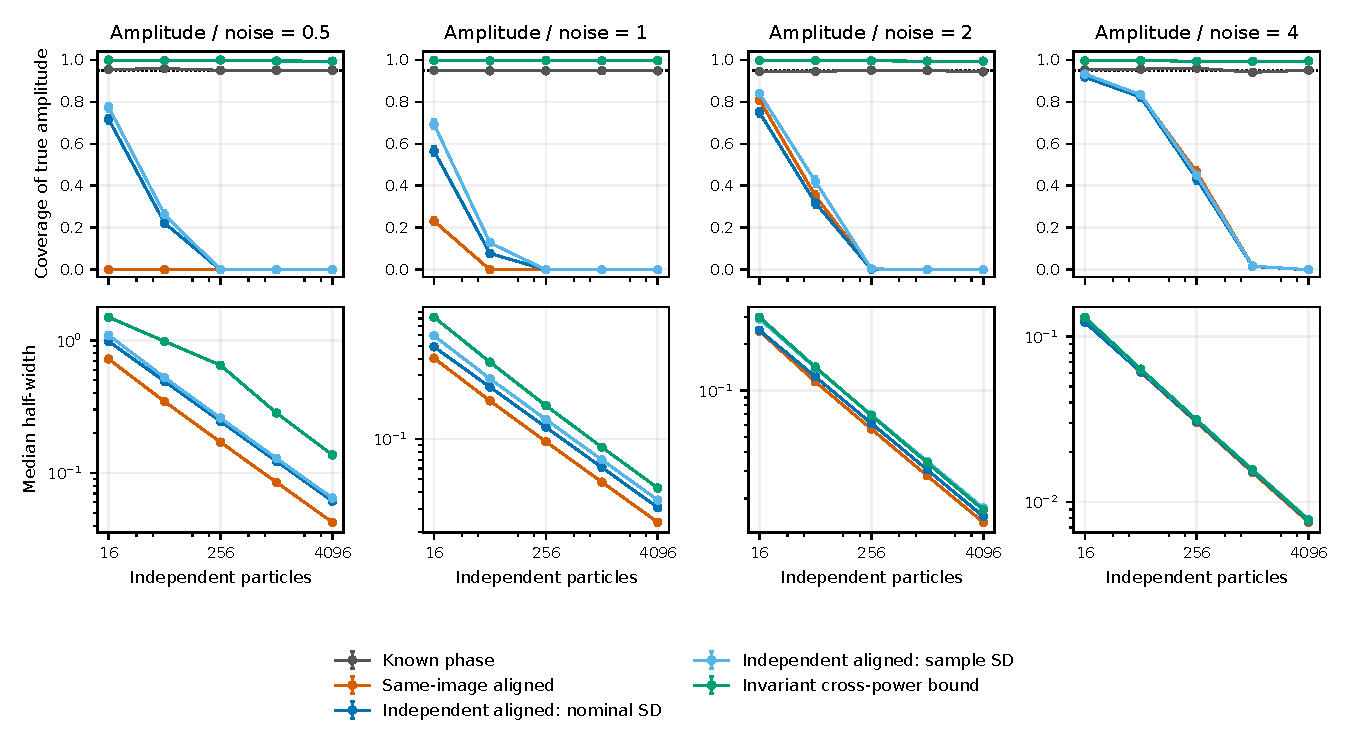
\includegraphics[width=\textwidth]{figures/phase-split-control.pdf}
\caption{Declared phase-only control: 2,000 independent datasets per case,
five paired procedures, four amplitude-to-coordinate-noise ratios, and five
particle counts. At 4,096 particles all three naive aligned intervals have
zero observed coverage in every noise setting. Independent-image sample
variance does not correct attenuation. Oracle coverage is near .95; the
invariant concentration interval is conservative. Width and coverage are
both retained. This is a one-frequency mechanism diagnostic with known
noise, not a reconstruction benchmark.}
\label{fig:phasecontrol}
\end{figure*}
